\section{Test of the Baseline Algorithm}
\begin{enumerate}
\item Test the algorithm for the toy example
	\begin{itemize}
	\item Test for $M = 8$ and varying $N = 8, 16, 32$. Plot the errors in the same plot.
	\item Test for $M = 16$ and varying $N = 16, 32$. Plot the errors in the same plot.
	\item Compare the errors with the errors achieved with the real A
	\end{itemize}	 
\item Test the algorithm for the AR data
	\begin{itemize}
	\item Test for $M = 8$ and varying $N = 8, 16, 32$. Plot the errors in the same plot.
	\item Test for $M = 16$ and varying $N = 16, 32$. Plot the errors in the same plot.
	\item Compare the errors with the errors achieved with the real A
	\end{itemize}	
\end{enumerate}   

A = array([1.9430682 , 2.16890318, 2.05233559])
X = array([420.88522225,   8.379144  ,   7.5566646 ])
\begin{figure}[H]
\centering
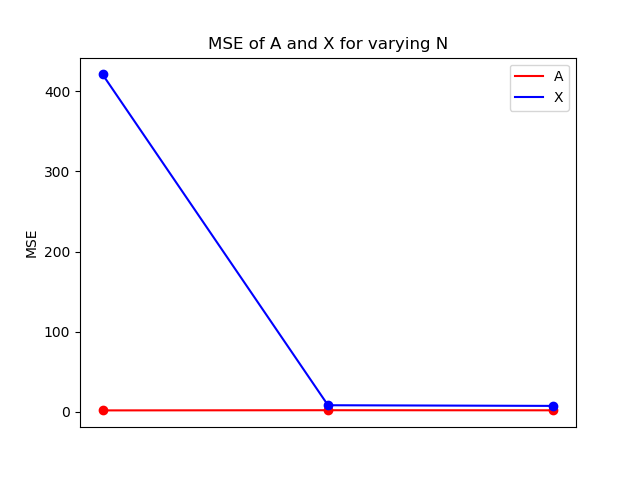
\includegraphics[scale=0.5]{figures/chapter6/AR_Error_vary_n_m8_L1000.png}
\caption{.}
\label{fig:}
\end{figure}
\noindent


A = array([1.96434494, 1.97380226])
X = array([691.21035395,  10.51375361])
\begin{figure}[H]
\centering
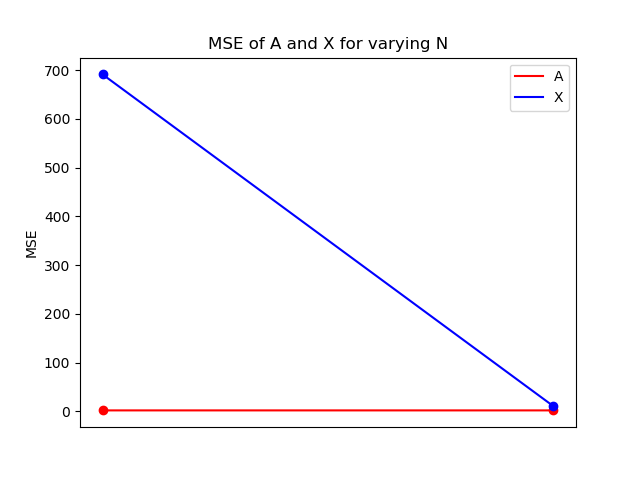
\includegraphics[scale=0.5]{figures/chapter6/AR_Error_vary_n_m16_L1000.png}
\caption{.}
\label{fig:}
\end{figure}
\noindent
\todo[inline]{opbygning ud fra mine noter:\\
intro \\
implementering \\
beskrivele af simuleret data\\
N=k diskussion\\
test af A på toy,test af X på toy(lidt i tvivl her måske de godt kan slås sammen med AR)\\
test af A på AR, test af init og cov-seg\\
samlet test på AR}